\chapter{Experiments}\label{action-space-experiments}

\section{Interfaces}




\section{n-dimensional Cart pole}

\begin{displayquote}
  \textit{How can we test a learners ability to detect symmetries and exploit them?}
\end{displayquote}

We propose a simple test, the n-dimensional cart pole: a generalisation of the
cart pole problem to $n$ dimensions. Rather than receiving observations in
$\mathbb{R}^4$ (the position, velocity, angle and angular velocity), observations are
in $\mathbb{R}^{4\times n}$. And the action space is generalised from $\{0,1\}$ (left and right),
to $\{0,1\}^{n}$.

\cite{Brockman2016,baselines}

% What makes this problem hard??

% Existing envs dont test this because!?!?

\subsection{How is this problem symmetric?}

Well, the original cart pole problem has a few symmetries in it. But these are
not central to the ...

Many people realise that this problem can be reduce to $n$, one dimensional cart pole problems.
But the learner needs to infer that.

More formally. How does this problem have symmetry?
Permutations of the observation-action space preserve the problem.

\subsection{How might a learner exploit this knowledge to learn more efficiently?}

What advantage is provided by this knowledge?

If we knew that the problem can be decomposed into $n$ identical subproblems,
then that means we are gathering $n$ times the data for each subproblem.
So, we should see a factor of $n$ speed up in learning.

This is the same argument made here [quotient groups appendix...].

For a learner that doesn't know of the symmetries. How is this problem hard?
The more dimensions there are, the more ways there are to fail.
Consider how exploration is done. In a single dimension, a greedy action is
taken with some chance of exploring instead.

Maybe you correctly balanced the pole in all dimensions except one. To bad, you dont get any reward.



\subsection{Experiments}

What about if we rotate the observations. So the observations are not aligned with the actions?
Or generalising to n+1? Could start the agent off with n+1 dims. But set them to observe nothing / actions do nothing. Until t > T?

\begin{figure}
  \centering
  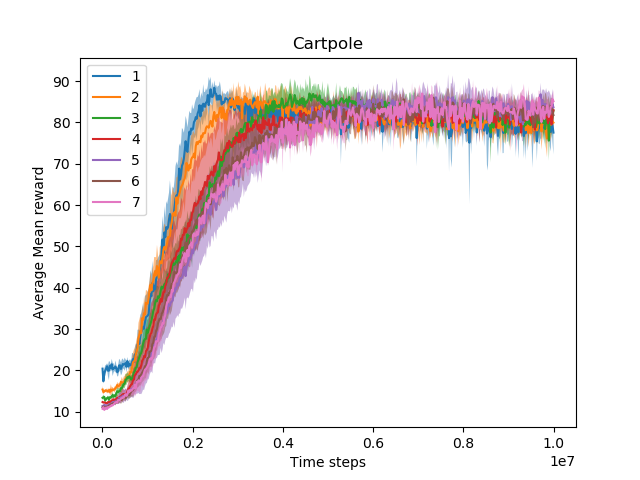
\includegraphics[width=1\textwidth,height=0.5\textheight]{../../pictures/figures/multibinary-nd-cart.png}
  \caption{PPO2 solving the nd cartpole problem with access to a \textit{MultiBinary} action space that grows with $N$.}
\end{figure}

\begin{figure}
\centering
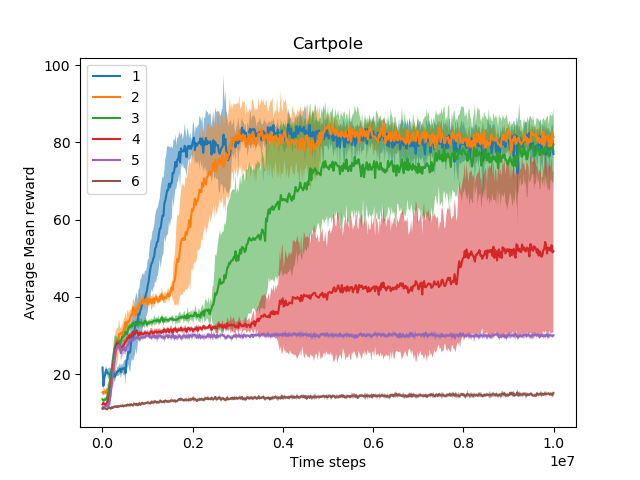
\includegraphics[width=1\textwidth,height=0.5\textheight]{../../pictures/figures/discrete-nd-cart.png}
\caption{PPO2 solving the nd cartpole problem with access to a \textit{Discrete} action space that grows with $2^N$.}
\end{figure}


\textit{Note: Average mean reward refers to the fact that we have averaged (n=5)
the mean reward (per episode). Also, this reward is the training performance.
Generalisation in RL can mean a few things.}

It seems surprising that access to the \textit{MultiBinary} action space provides such an advantage.
Also, it seems surprising that the an increase of 6 dimensions only results in approximately a ~2 million increase in the data required.
Is the learner doing some sort of intelligent sharing?
Why is it so hard for the Discrete learner? What operation does it find hard to learn. The ability to decode? $n$ bits to $2^n$ onehots?

Also, interesting to note that the 1D learner equipped with a \textit{Discrete}
action space achieves max performance at ~1.75 million samples, while the learner
equipped with a \textit{MultiBinary} action space achieves max performance at ~2.25 million samples. (significant??)
